\section*{External delay optimization}
\blankpage
\section*{Analog Time resolution as function of energy}
In order to study the time resolution dependence as a function of energy a different radioactive source, $^{60}$Co, was used. This source is chosen because of its high energy Compton Edge ($\approx$1~MeV) that allows to study the energy dependence up to this value. 

Two methods were used to characterize the  timing resolution for different energies: 
\begin{itemize}
	\item Energy Windows
	\item Energy Thresholds
\end{itemize} 

\subsection*{Energy Windows}
 The analog timing distributions were produced selecting events inside energy windows of 100~keV width in the range 100~keV-1~MeV~(see~Fig.~\ref{Fig:Energy_slice}). 
\begin{figure}[h!]
	\centering
	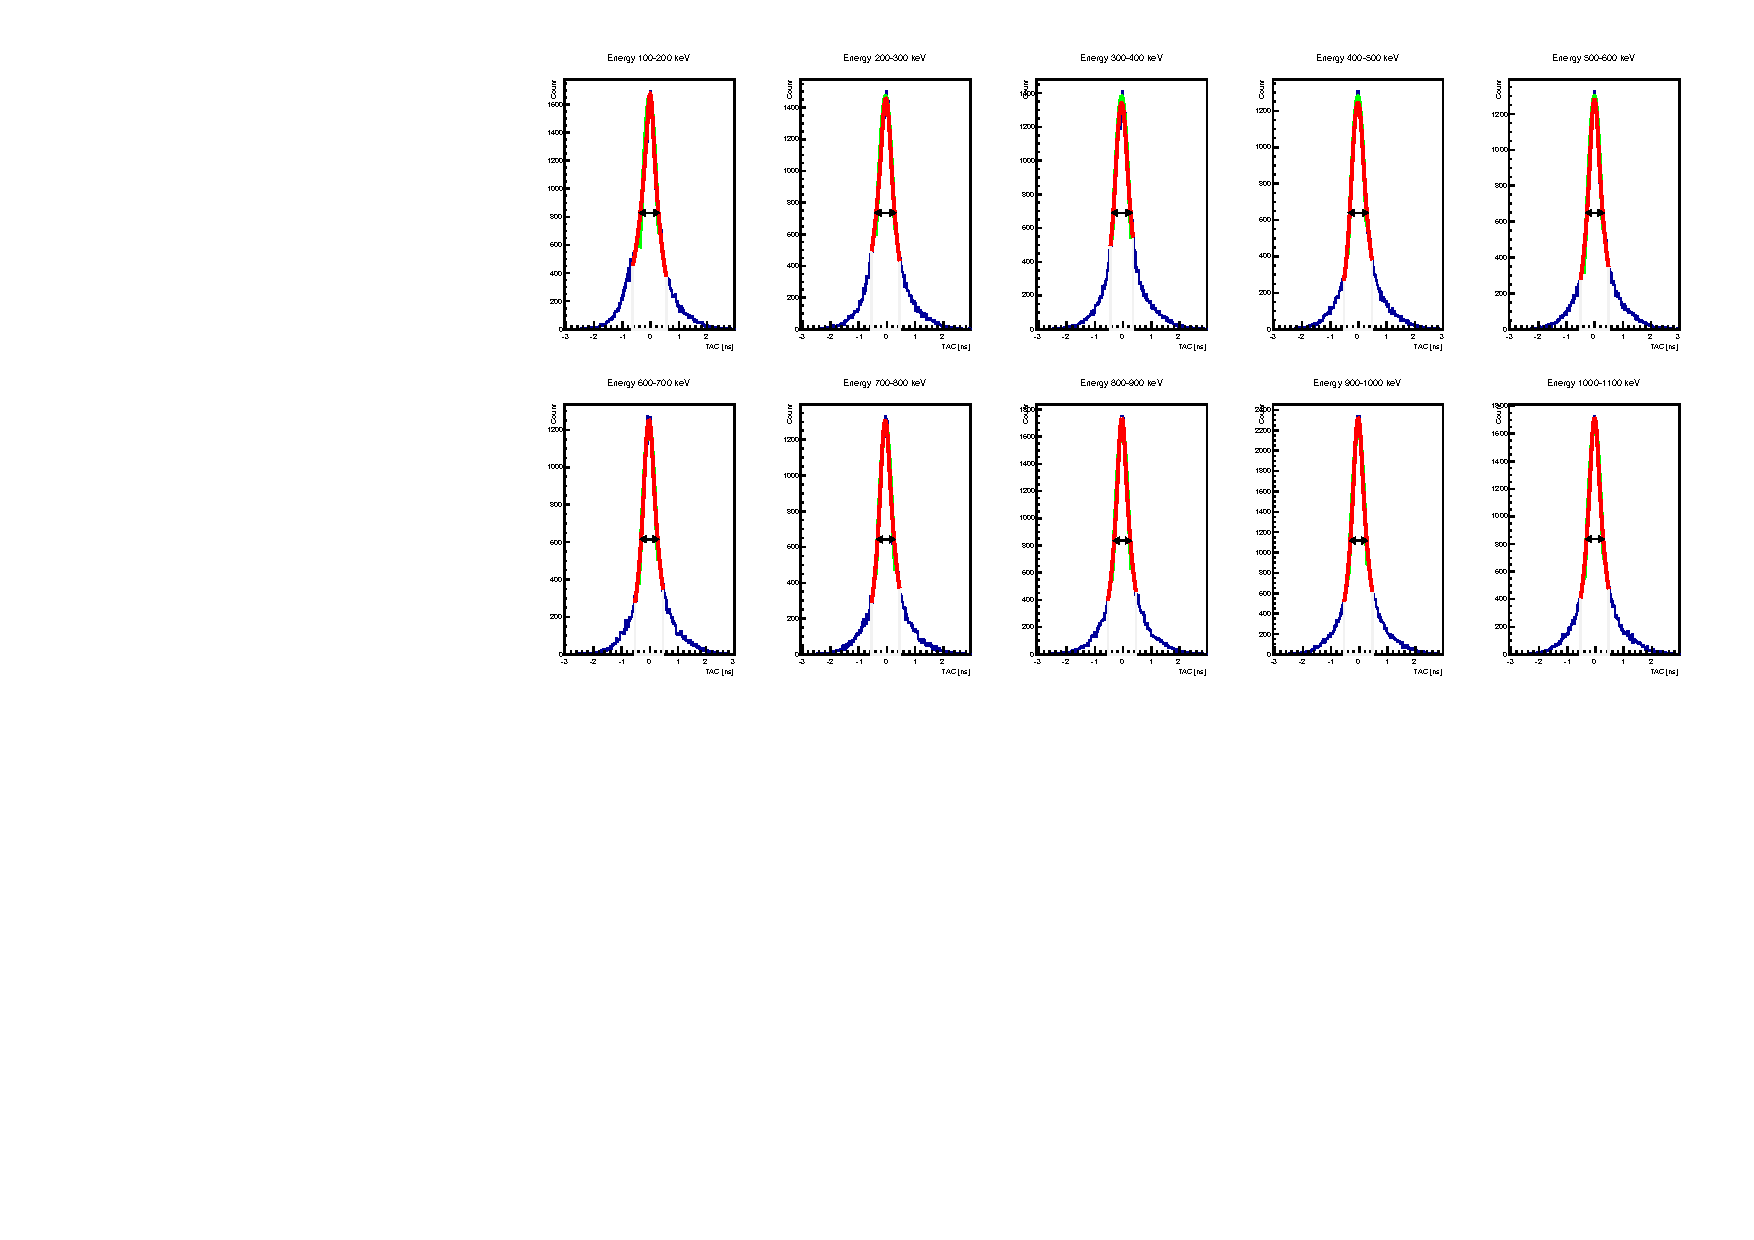
\includegraphics[width = \textwidth]{SlicedTACdists}
	\caption{Timing distributions obtained selecting events inside 100~keV energy windows.}
	\label{Fig:Energy_slice}
\end{figure}

For each distribution the FWHM was computed and reported in the Fig.~\ref{fig: energy windows analog} below, over the 2-D density plot of timing as function of energy.

\begin{figure}[h!]
	\centering
	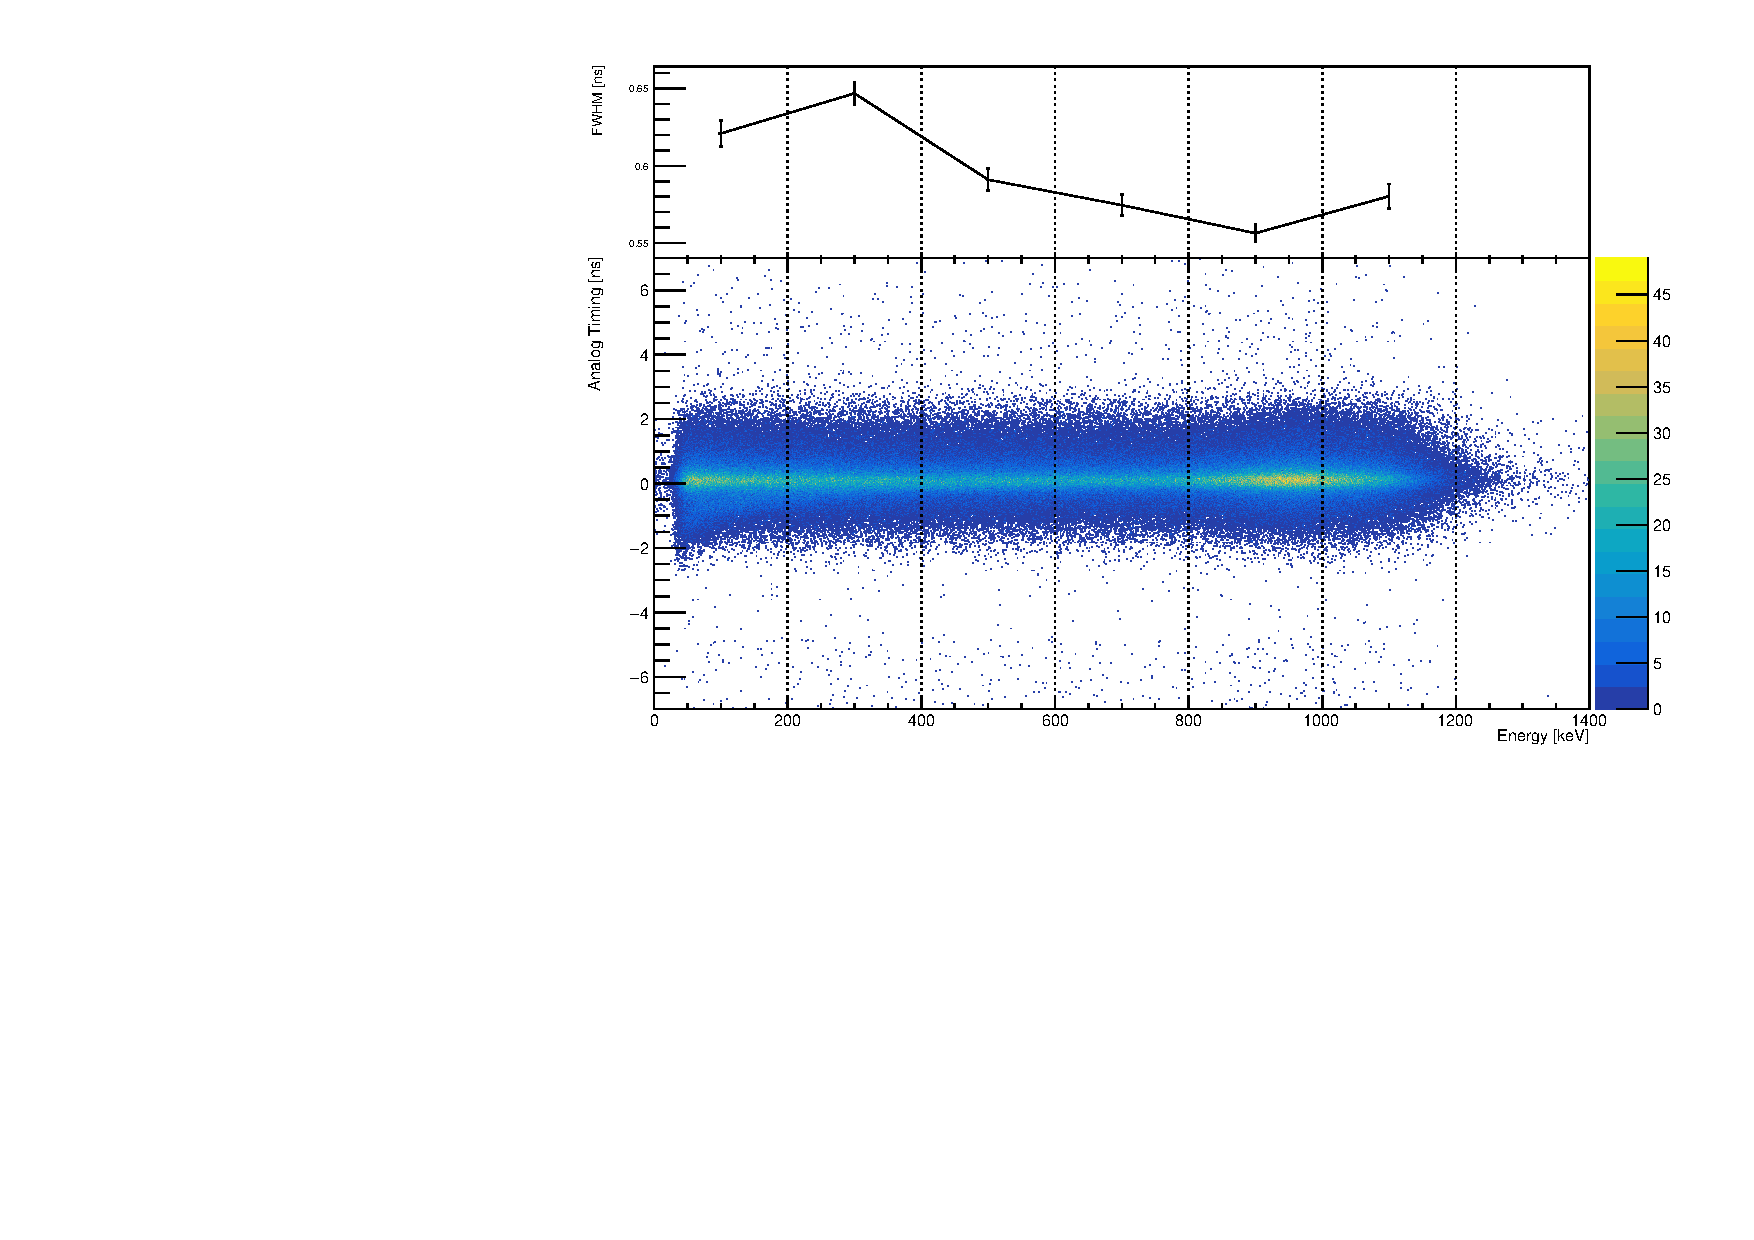
\includegraphics[width = \textwidth]{SlicedTAC_FWHMvs2Ddist}
	\caption{FWHM for each energy slice over 2-D density plot of timing as function of energy. }
	\label{fig: energy windows analog}
\end{figure}
\newpage

\subsection*{Energy Threshold}
 The analog timing distributions were produced selecting events by mean of different energy thresholds from 100~keV to 1~MeV~(see~Fig.~\ref{Fig: lower energy thr}). 

\begin{figure}[H]
	\centering
	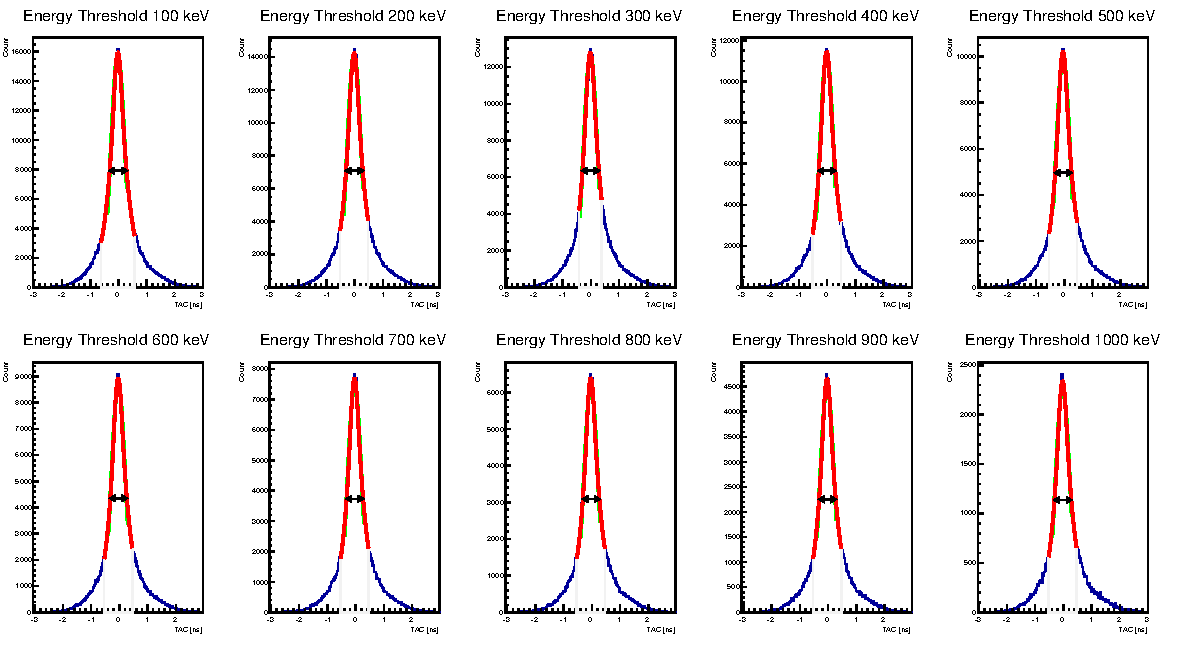
\includegraphics[width = \textwidth]{ThresholdTAC_dists}
	\caption{Timing distributions obtained selecting events inside by mean of different energy thresholds.}
	\label{Fig: lower energy thr}
\end{figure}
\newpage
In the same way, for each distribution, the FWHM was computed and reported in the Fig.~\ref{Fig:2Dplot_th} below:

\begin{figure}[H]
	\centering
	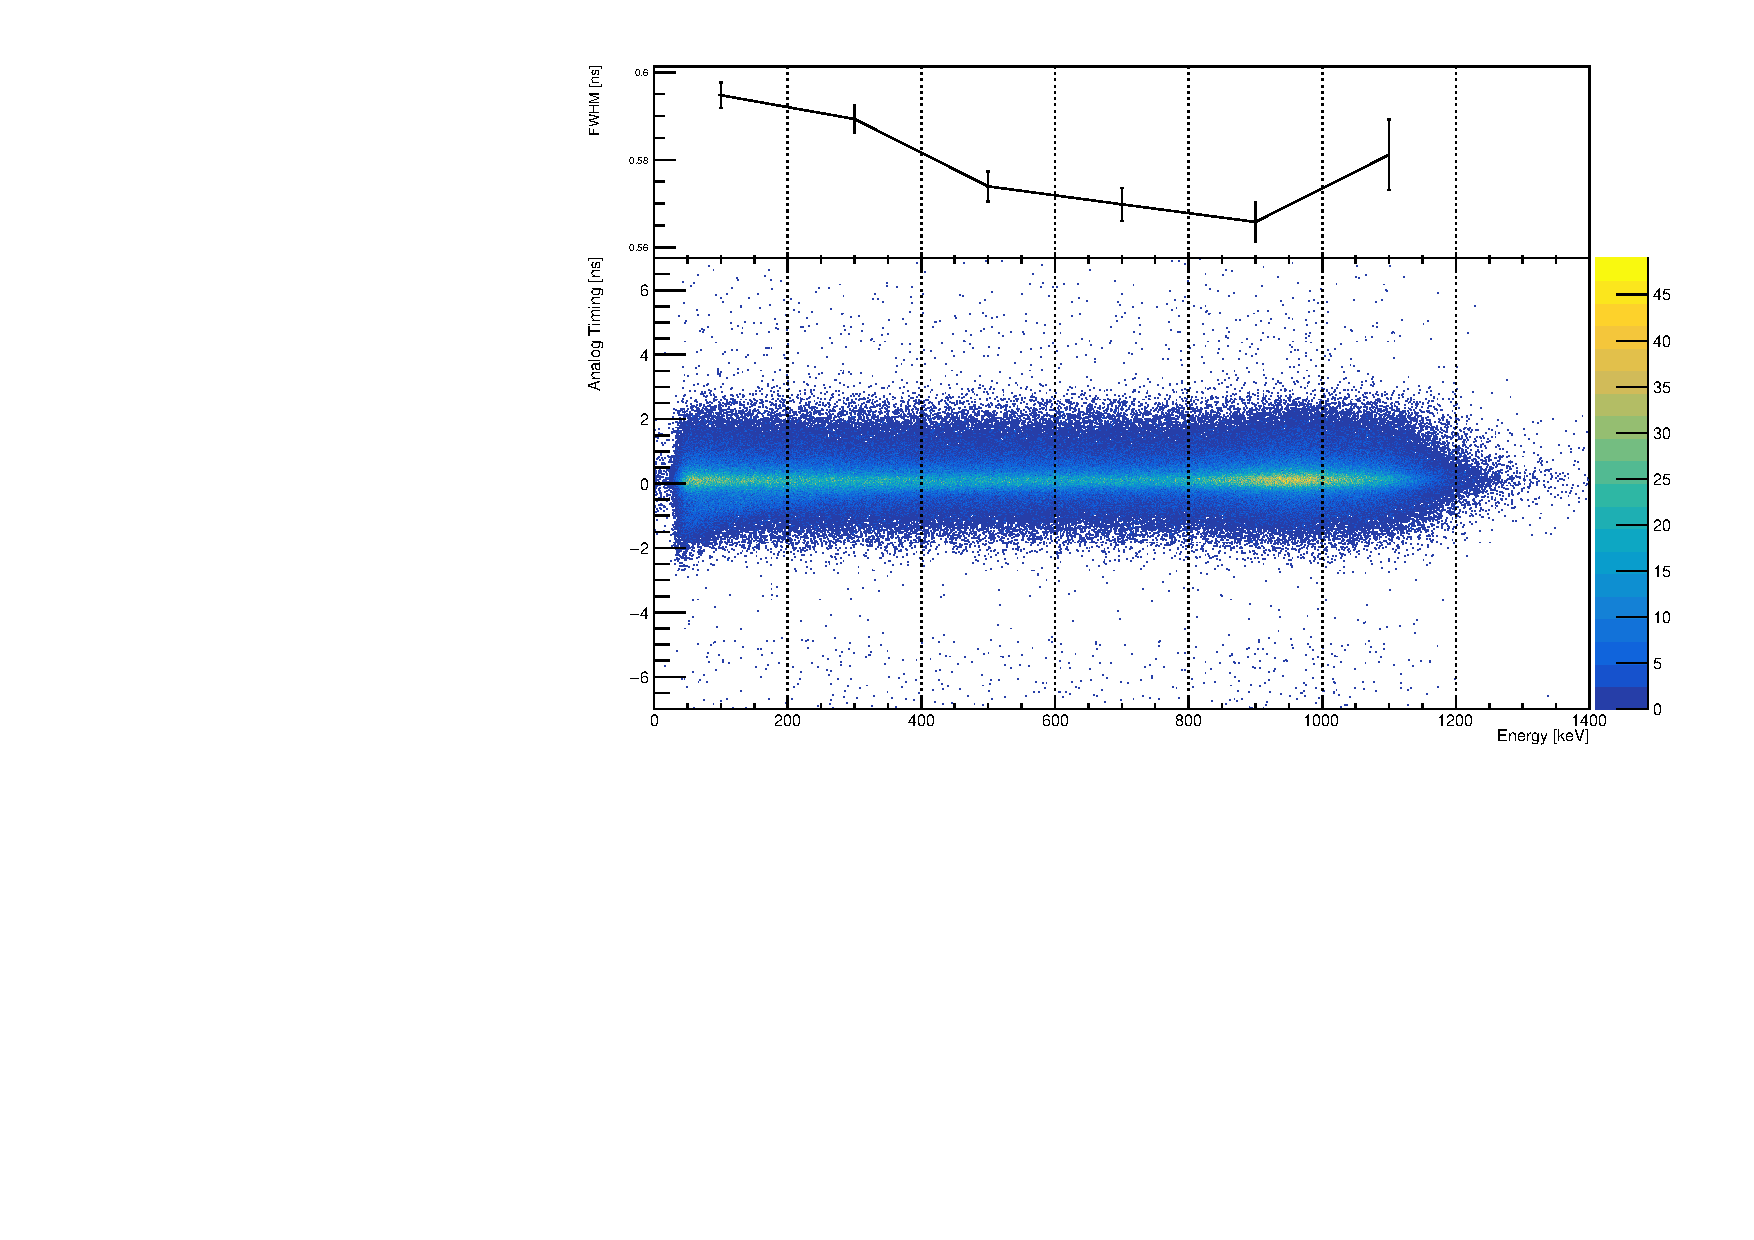
\includegraphics[width = 1\textwidth]{ThresholdTAC_FWHMvs2Ddist}
	\caption{Lower energy threshold.}
	\label{Fig:2Dplot_th}
\end{figure}

\subsection*{Methods  comparison}

The overlay of the FWHM obtained with the two methods is presented in Fig.~\ref{Fig:Slice_th_comp}. Both the curves show a minimum around the Compton edge of the spectrum, while for greater energies the increasing of FWHM could be explained by mean of multi-scattering interactions inside the detectors. The errors associated to the values, for threshold method, increase with energy. Instead for windows methods decrease moving to the Compton edge. %%%%%%%%%%%%%%%%%%%%rivedi


\begin{figure}[H]
	\centering
	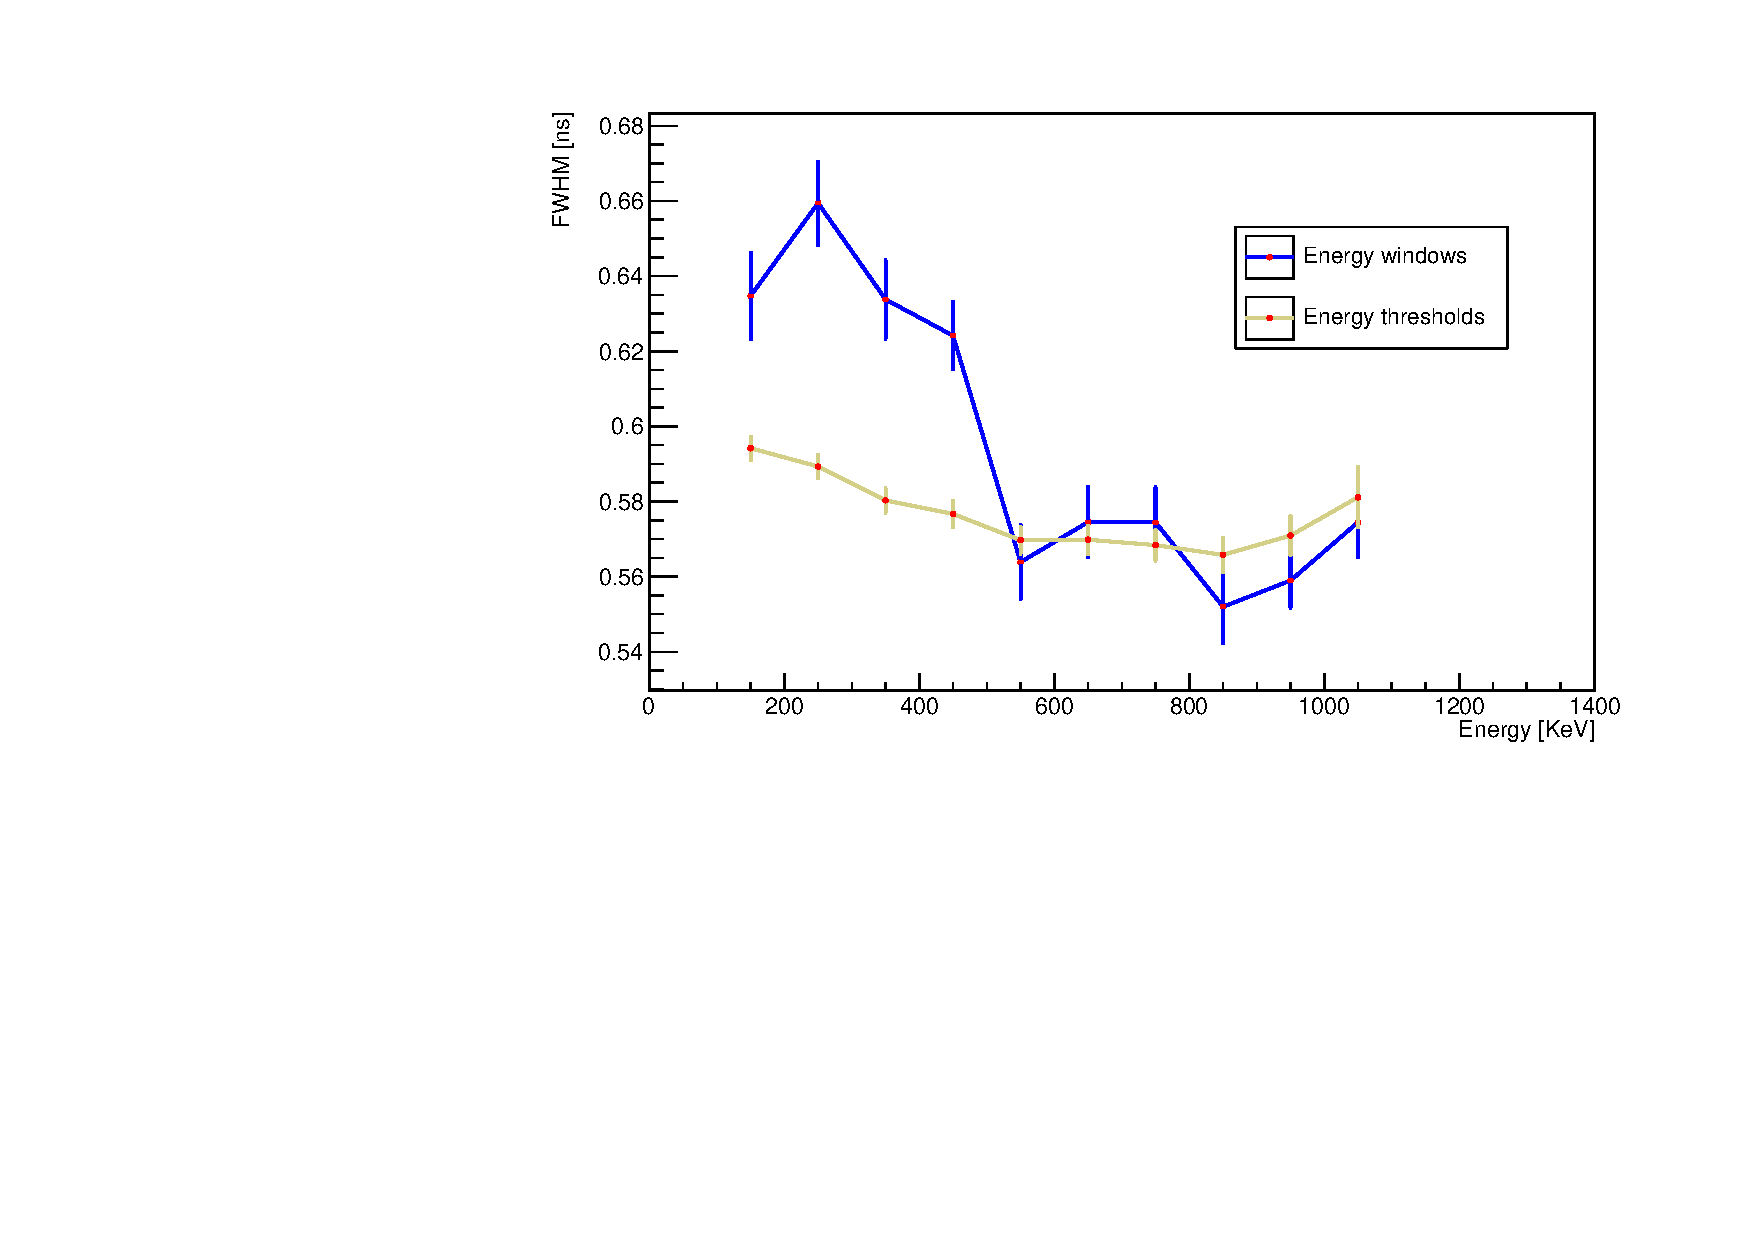
\includegraphics[width = 1\textwidth]{Slice_thresh_comparison}
	\caption{FWHM obtained from different energy windows and different energy thresholds compared.}
	\label{Fig:Slice_th_comp}
\end{figure}










